%%%%%%%%%%%%%%%%%%%%%%%%%%%%%%%%%%%%%%%%%
% Beamer Presentation
% LaTeX Template
% Version 1.0 (10/11/12)
%
% This template has been downloaded from:
% http://www.LaTeXTemplates.com
%
% License:
% CC BY-NC-SA 3.0 (http://creativecommons.org/licenses/by-nc-sa/3.0/)
%
%%%%%%%%%%%%%%%%%%%%%%%%%%%%%%%%%%%%%%%%%

%----------------------------------------------------------------------------------------
%	PACKAGES AND THEMES
%----------------------------------------------------------------------------------------

\documentclass[8pt]{beamer}

\mode<presentation> {

% The Beamer class comes with a number of default slide themes
% which change the colors and layouts of slides. Below this is a list
% of all the themes, uncomment each in turn to see what they look like.

%\usetheme{default}
%\usetheme{AnnArbor}
%\usetheme{Antibes}
%\usetheme{Bergen}
\usetheme{Berkeley}
%\usetheme{Berlin}
%\usetheme{Boadilla}
%\usetheme{CambridgeUS}
%\usetheme{Copenhagen}
%\usetheme{Darmstadt}
%\usetheme{Dresden}
%\usetheme{Frankfurt}
%\usetheme{Goettingen}
%\usetheme{Hannover}
%\usetheme{Ilmenau}
%\usetheme{JuanLesPins}
%\usetheme{Luebeck}
%\usetheme{Madrid}
%\usetheme{Malmoe}
%\usetheme{Marburg}
%\usetheme{Montpellier}
%\usetheme{PaloAlto}
%\usetheme{Pittsburgh}
%\usetheme{Rochester}
%\usetheme{Singapore}
%\usetheme{Szeged}
%\usetheme{Warsaw}

% As well as themes, the Beamer class has a number of color themes
% for any slide theme. Uncomment each of these in turn to see how it
% changes the colors of your current slide theme.

%\usecolortheme{albatross}
%\usecolortheme{beaver}
%\usecolortheme{beetle}
%\usecolortheme{crane}
%\usecolortheme{dolphin}
%\usecolortheme{dove}
%\usecolortheme{fly}
%\usecolortheme{lily}
%\usecolortheme{orchid}
%\usecolortheme{rose}
%\usecolortheme{seagull}
%\usecolortheme{seahorse}
%\usecolortheme{whale}
%\usecolortheme{wolverine}

%\setbeamertemplate{footline} % To remove the footer line in all slides uncomment this line
\setbeamertemplate{footline}[page number] % To replace the footer line in all slides with a simple slide count uncomment this line

%\setbeamertemplate{navigation symbols}{} % To remove the navigation symbols from the bottom of all slides uncomment this line
}

\usepackage{graphicx} % Allows including images
\usepackage{booktabs} % Allows the use of \toprule, \midrule and \bottomrule in tables
\usepackage{tabularx}  % for 'tabularx' environment and 'X' column type
\usepackage{ragged2e}  % for '\RaggedRight' macro (allows hyphenation)
\newcolumntype{Y}{>{\RaggedRight\arraybackslash}X} 

\setcounter{figure}{0}

%----------------------------------------------------------------------------------------
%	TITLE PAGE
%----------------------------------------------------------------------------------------

\title[Evolutionary Robotics\\An Overview]{Evolutionary Robotics\\-\\An Overview} % The short title appears at the bottom of every slide, the full title is only on the title page
\author{Bastian Lang} % Your name
\institute[BRSU] % Your institution as it will appear on the bottom of every slide, may be shorthand to save space
{
Master of Autonomous Systems \\ % Your institution for the title page
}
\date{April 6, 2015} 

\begin{document}


\listoffigures
\begin{frame}
\titlepage 
\end{frame}

%----------------------------------------------------------------------------------------
%	PRESENTATION SLIDES
%----------------------------------------------------------------------------------------

\begin{frame}
\frametitle{Evolutionary Robotics\\Overview}
\begin{itemize}
\item Technique for the automatic creation of autonomous robots
\item Inspired by darwinian principle of selective reproduction of the fittest
\item Use of evolutionary algorithms and artificial neural networks
\item Three major trends
	\begin{itemize}
	\item Parameter tuning/ Neuroevolution
		\begin{itemize}
		\item Use EA to tune parameters
		\end{itemize}
	\item Online evolutionary adaptation
	\begin{itemize}
		\item Open-ended
	\end{itemize}
	\item Evolutionary synthesis
		\begin{itemize}
		\item Body-brain evolution
		\end{itemize}
	\end{itemize}

\item Tools
	\begin{itemize}
	\item Evolutionary Algorithms
	\item Simulated evolution
	\item Embodied evolution
	\end{itemize}
\end{itemize}
\end{frame}

\begin{frame}
\frametitle{Mindmap}
\begin{figure}[ht]
	\centering
  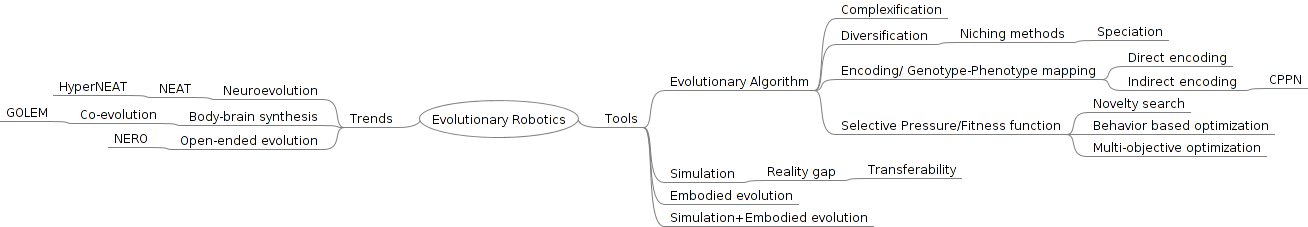
\includegraphics[width=1\textwidth]{Evolutionary_Robotics_151013.png}
	\caption{Mindmap ER}
	\label{fig1}
\end{figure}
\end{frame}

\begin{frame}
\frametitle{Fundamental Problems}
\begin{itemize}
	\item Neuroevolution
	\begin{itemize}
		\item How to evolve neural networks for robot controlling tasks?
	\end{itemize}
	\item The Reality Gap
	\begin{itemize}
		\item Different behavior on real robot and on simulated one
	\end{itemize}
	\item How to apply selective pressure?
	\begin{itemize}
		\item How to evaluate an individual?
		\item What is a good fitness function?
		\item One goal vs multiple goals
		\item Behavior based
		\item Problems of fitness landscapes
	\end{itemize}
	
\end{itemize}
\end{frame}

\begin{frame}
\frametitle{Neuroevolution - Top 1 paper}
Stanley, K. O., \& Miikkulainen, R. (2002). Evolving neural networks through augmenting topologies. Evolutionary computation, 10(2), 99-127.
\begin{itemize}
	\item Problem formulation
	\begin{itemize}
		\item Artificial evolution of neural networks using genetic algorithms
	\end{itemize}
	\item Deficits of the state of the art
	\begin{itemize}
		\item Modifying structure of ANN has been efficient
		\item Fixed topologies
		\item Random initialization of hidden layers
	\end{itemize}		 
	\item Approach taken
	\begin{itemize}
		\item Global innovation number to make cross over possible
		\item Complexification 
		\item Fitness sharing for diverse populations
	\end{itemize}
	\item Evaluation and experimental results
	\begin{itemize}
		\item Create XOR gates and double pole balancing
		\item Comparison to best fixed structure methods so far $\rightarrow$ 8 times slower and not as successful
		\item Explicitly test for cross over, complexification and fitness sharing $\rightarrow$ More evaluations needed and loss of success rate
	\end{itemize}
\end{itemize}
\end{frame}

\begin{frame}
\frametitle{Neuroevolution - Top 6 list}
\begin{itemize}
	\item Stanley, K. O., \& Miikkulainen, R. (2002). Evolving neural networks through augmenting topologies. Evolutionary computation, 10(2), 99-127.
	\item Yao, X. (1999). Evolving artificial neural networks. Proceedings of the IEEE, 87(9), 1423-1447.
	\item Kashtan, N., \& Alon, U. (2005). Spontaneous evolution of modularity and network motifs. Proceedings of the National Academy of Sciences of the United States of America, 102(39), 13773-13778.
	\item Angeline, P. J., Saunders, G. M., \& Pollack, J. B. (1994). An evolutionary algorithm that constructs recurrent neural networks. Neural Networks, IEEE Transactions on, 5(1), 54-65.
	\item Clune, J., Beckmann, B. E., Ofria, C., \& Pennock, R. T. (2009, May). Evolving coordinated quadruped gaits with the HyperNEAT generative encoding. In Evolutionary Computation, 2009. CEC'09. IEEE Congress on (pp. 2764-2771). IEEE.
	\item Harvey, I., Husbands, P., Cliff, D., Thompson, A., \& Jakobi, N. (1997). Evolutionary robotics: the Sussex approach. Robotics and autonomous systems, 20(2), 205-224.
\end{itemize}
\end{frame}

\begin{frame}
\frametitle{Reality Gap - Top 1 Paper}

Koos, S., Mouret, J. B., \& Doncieux, S. (2013). The transferability approach: Crossing the reality gap in evolutionary robotics. Evolutionary Computation, IEEE Transactions on, 17(1), 122-145.

\begin{itemize}
	\item Problem formulation
	\begin{itemize}
		\item Optimal solutions found in simulation perform significantly less good on real robot
		\item Evolutionary algorithms exploiting faulty parts of simulations
		\item Evolution on real robots is very time consuming and not always possible
	\end{itemize}
	\item Deficits of the state of the art
	\begin{itemize}
		\item Evolution on real robots is too slow
		\item Assumptions that simulation optimum is similar to optimum in reality
		\item Very accurate simulations are hard to create and computationally costly
		\item Creating robust solutions will most likely end up in worse local optima
		\item Human needed to help identify the dynamic system		
	\end{itemize}		 
	\item Approach taken
	\begin{itemize}
		\item Create and update a surrogate model
		\item Use simulation-to-reality mapping as additional goal to drop solutions that exploit errors of simulation.
	\end{itemize}
	\item Evaluation and experimental results
	\begin{itemize}
		\item Two wheeled robot that had to turn into the right direction at a T-cross depending on some light signals
		\item Four-legged robot gait
		\item Compared to purely simulation based approach with small variations, two reality based approaches and a noise-based approach
		\item Simulation only performed much worse after transfer
		\item Real robot based approaches bad in the first, quite good in the second experiment
		\item Noise based approach better
		\item Transferability best
		\item Transferability does not correlate with robustness (behavior is not the same)
	\end{itemize}
\end{itemize}

\end{frame}

\begin{frame}
\frametitle{Reality Gap - Top 6 list}
\begin{itemize}
	\item Miglino, O., Lund, H. H., \& Nolfi, S. (1995). Evolving mobile robots in simulated and real environments. Artificial life, 2(4), 417-434.
	\item Jakobi, N., Husbands, P., \& Harvey, I. (1995). Noise and the reality gap: The use of simulation in evolutionary robotics. In Advances in artificial life (pp. 704-720). Springer Berlin Heidelberg.
	\item Koos, S., Mouret, J. B., \& Doncieux, S. (2013). The transferability approach: Crossing the reality gap in evolutionary robotics. Evolutionary Computation, IEEE Transactions on, 17(1), 122-145.
	\item Jakobi, N. (1998, January). Running across the reality gap: Octopod locomotion evolved in a minimal simulation. In Evolutionary Robotics (pp. 39-58). Springer Berlin Heidelberg.
	\item Hartland, C., \& Bredeche, N. (2006, December). Evolutionary robotics, anticipation and the reality gap. In Robotics and Biomimetics, 2006. ROBIO'06. IEEE International Conference on (pp. 1640-1645). IEEE.
	\item Toris, R. (2011). Evolving Robotic Desires: A New Approach to Bridging the Reality Gap (Doctoral dissertation, Dickinson College).
\end{itemize}
\end{frame}

\begin{frame}
\frametitle{Fitness functions and selective pressure - Top 1 paper}
Lehman, J., \& Stanley, K. O. (2011). Abandoning objectives: Evolution through the search for novelty alone. Evolutionary computation, 19(2), 189-223.
\begin{itemize}
	\item Problem formulation
	\begin{itemize}
		\item Measuring progress
		\item Strategies to explore the search space
		\item Fitness functions usually used for this
	\end{itemize}
	\item Deficits of the state of the art
	\begin{itemize}
		\item Increasing fitness does not always reveal the best path through the search space		
		\item Objectives may lead to local optima
		\item The more complex the goal, the harder to formulate
		\item May ignore step stones to optimal solution
	\end{itemize}		 
	\item Approach taken
	\begin{itemize}
		\item Fitness based on novelty of behavior
		\item Combined with NEAT solutions become more and more complex
		\item Use metric to compute novelty as distance to other solutions
		\item Keep track of all novel solutions
	\end{itemize}
	\item Evaluation and experimental results
	\begin{itemize}
		\item Compare novelty search to objective and random search
		\item Two maps containing deceptive dead ends
		\item First map novelty needed significantly less evaluations than NEAT with objective
		\item Second map NEAT 3 out of 50, novelty 49 out of 50
	\end{itemize}
\end{itemize}
\end{frame}

\begin{frame}
\frametitle{Fitness functions and selective pressure - Top 6 list}
\begin{itemize}
	\item Lehman, J., \& Stanley, K. O. (2011). Abandoning objectives: Evolution through the search for novelty alone. Evolutionary computation, 19(2), 189-223.
	\item Nelson, A. L., Barlow, G. J., \& Doitsidis, L. (2009). Fitness functions in evolutionary robotics: A survey and analysis. Robotics and Autonomous Systems, 57(4), 345-370.
	\item Sareni, B., \& Krähenbühl, L. (1998). Fitness sharing and niching methods revisited. Evolutionary Computation, IEEE Transactions on, 2(3), 97-106.
	\item Mouret, J. B., \& Doncieux, S. (2012). Encouraging behavioral diversity in evolutionary robotics: An empirical study. Evolutionary computation, 20(1), 91-133.
	\item Jin, Y., Olhofer, M., \& Sendhoff, B. (2002). A framework for evolutionary optimization with approximate fitness functions. Evolutionary Computation, IEEE Transactions on, 6(5), 481-494.
	\item Jin, Y., Olhofer, M., \& Sendhoff, B. (2000, July). On Evolutionary Optimization with Approximate Fitness Functions. In GECCO (pp. 786-793).
\end{itemize}
\end{frame}





\end{document} 